\documentclass[
%a4paper,12pt
encoding=utf8
]{./twoeskd}

% \usepackage{eskdappsheet}

% Packages required by doxygen
\usepackage[export]{adjustbox} % also loads graphicx
%\usepackage[utf8]{inputenc}
\usepackage{multicol}
\usepackage{multirow}
\usepackage{makeidx}
\usepackage{caption}
\usepackage{graphicx}



% NLS support packages
\usepackage[T2A]{fontenc}
\usepackage[russian]{babel}
\usepackage{pscyr}

% Font selection
\usepackage{courier}
\usepackage{amssymb}

% Page & text layout
% \usepackage{geometry}
% \geometry{%
%   a4paper,%
%   top=2.5cm,%
%   bottom=4.5cm,%
%   left=2.5cm,%
%   right=2.5cm%
% }
%\setlength{\emergencystretch}{15pt}
\setlength{\parindent}{0cm}
\setlength{\parskip}{0.2cm}

% Headers & footers
% \usepackage{fancyhdr}
% \pagestyle{fancyplain}
% \fancyhead[L]{\fancyplain{}{}}
% \fancyhead[C]{\fancyplain{}{\scriptsize\textbf{RU.17701729.509000 ТЗ 01-1-ЛУ}}}
% \fancyhead[R]{\fancyplain{}{}}
% \fancyfoot[L]{\fancyplain{}{}}
% \fancyfoot[C]{\fancyplain{}{}}
% \fancyfoot[R]{\fancyplain{}{}}

% debug to see the frame borders
% from https://en.wikibooks.org/wiki/LaTeX/Page_Layout
% \usepackage{showframe}

% Indices & bibliography
\usepackage[backend=biber
           % ,style=authoryear-icomp
            ]{biblatex}
\addbibresource{used_sources.bib}
\usepackage[titles]{tocloft}
\setcounter{tocdepth}{3}
\setcounter{secnumdepth}{5}


\newcommand\tab[1][1cm]{\hspace*{#1}}

% change style of titles in \section{}
\usepackage{titlesec}
\titleformat{\section}[hang]{\huge\bfseries\center}{\thetitle.}{1em}{}
\titleformat{\subsection}[hang]{\Large\normalfont\raggedright}{\thetitle.}{1em}{\underline}
\titleformat{\subsubsection}[hang]{\large\normalfont\raggedright}{\thetitle.}{1pt}{}

% Packages for text layout in normal mode
% \usepackage[parfill]{parskip} % автоматом делает пустые линии между параграфами, там где они есть в тексте
% \usepackage{indentfirst} % indent even in first paragraph
\usepackage{setspace}	 % controls space between lines
\setstretch{1} % space between lines
\setlength\parindent{0.9cm} % size of indent for every paragraph
\usepackage{csquotes}% превратить " " в красивые двойные кавычки
\MakeOuterQuote{"}


% this makes items spacing single-spaced in enumerations.
\newenvironment{my_enumerate}{
\begin{enumerate}
  \setlength{\itemsep}{1pt}
  \setlength{\parskip}{0pt}
  \setlength{\parsep}{0pt}}{\end{enumerate}
}


% Custom commands
% configure eskd
\titleTop{
	{\Large ПРАВИТЕЛЬСТВО РОССИЙСКОЙ ФЕДЕРАЦИИ \\
		НАЦИОНАЛЬНЫЙ ИССЛЕДОВАТЕЛЬСКИЙ УНИВЕРСИТЕТ \\
		«ВЫСШАЯ ШКОЛА ЭКОНОМИКИ» } \\
	\vspace*{0.2cm}
	{Факультет компьютерных наук \\
		Департамент программнoй инженерии \\
	}
}
\titleDesignedBy{Студент группы БПИ 151 НИУ-ВШЭ}{Куприянов К. И.}

\titleAgreedBy{
	\parbox[t]{7cm} {
		\centerline{Академический руководитель ОП}
		\centerline{Системная и программная инженерия}
		\centerline{профессор ДПИ}
}}{Д.В. Александров}
\titleApprovedBy{
	\parbox[t]{7cm} {
		\centerline{Академический руководитель}
		\centerline{образовательной программы}
		\centerline{«Программная Инженерия»}
		\centerline{профессор, канд. техн. наук}
}}{В. В. Шилов}
\titleName{Клиент-Серверное Android-Приложение для Управления Скидками в Розничных Сетях}
\workTypeId{RU.17701729.506900 51 01-1}

\titleSubname{Программа и методика испытаний}

% Custom packages
\usepackage{pdfpages}

\makeindex

%===== C O N T E N T S =====


\begin{document}
% Titlepage & ToC
\pagenumbering{roman}

% some water filling text, that is pointless but adds text
% Технология блокчейн обычно ассоциируется с криптовалютой биткойн, потому что
биткойн - первая повсеместно используемая система, использующая блокчейн как
основу. По мере развития технологий число различных блокчейнов со множеством
способов их приложения резко возросло. Факт существования такого значительного
их количества можно объяснить тем, что при их реализации могут варьироваться
используемые криптографические алгоритмы и протоколы. В связи с этим возникла
проблема отсутствия систематически собранной и структурированной информации о
криптографических алгоритмах и протоколах в существующих распределенных
реестрах. Целью данной работы является сбор и классификация по использованию в
реестрах известных и распространенных на сегодняшний день криптографических
алгоритмов и протоколов. А в качестве программной составляющей проекта ---
инструмент, позволяющий создать персональный распределенный реестр в
образовательных или прикладных целях. Это библиотека на языке Python3.6, в
которой реализована имплементация блокчейна, а так же собраны реализации
рассмотренных алгоритмов.\\

\textbf{Ключевые слова} --- блокчейн, биткоин, распределённый реест,
технология распределённого реестра, криптография, классификация, Python.


\newpage
\pagenumbering{arabic}
\tableofcontents
% \pagenumbering{arabic}

% --- add my custom headers ---
\newpage
\section{Объект испытаний}
\subsection{Наименование программы}
Наименование программы на русском:
``Криптографические алгоритмы и протоколы для распределенных реестров''. \\
Наименование на английском:
``Cryptographic Algorithms and Protocols for Distributed Ledgers''. \\


\subsection{Краткая характеристика}
Программа предназначена для пользователей машин на семействе ОС GNU/Linux.
Цель работы --- создать удобное приложение для автоматизации программирования,
которое генерировало бы готовый код блокчейна с использованием алгоритмов,
выбранных пользователями.

Данный продукт будет служить ``инструментарием'' для программиста или любого
другого интересующегося криптографическими алгоритмами и протоколами, который
имел бы потребность интегрировать блокчейн в своё приложение (регистрация
гостей в отеле, социальную сеть, переводы, учёт документов). Так же программа
будет полезна людям, которые хотят узнать как работают современные
распределённые реестры с рассмотренными
аспектами. Это позволит быстро получать необходимую техническую информацию,
которую с трудом можно найти в общем доступе. Программа должна предоставлять не
только генерацию кода, но и дружелюбный интерфейс командной строки, в которой
форматирование и подсветка не будут сбивать с толку неподготовленного
пользователя.\\

Главной чертой данного приложения является самоподдерживаемая система по работе
с исходными кодами алгоритмов, расположенными удалённо. А так же лёгкая,
быстрая масштабируемость и модульность программного кода.

Приложение состоит из двух компонент:
\begin{enumerate}
    \item Позволяющей сгенерировать код блокчейна с использованием выбранных
          пользователем алгоритмов
    \item Является выходом первой компоненты, и по своей сути обособленным приложением --- блокчейном
\end{enumerate}

В дальнейшем (1) будет именоваться \textbf{компоновщик}, а (2) --- \textbf{реализация блокчейна}. 


\newpage
\section{Цель испытаний}
Цель проведения испытаний заключается в проверке выполнения заявленных в
техническом задании требований к программной документации и составу выполняемых
функций программы, надежности и корректности ее работы, а также интерфейсу и
внешнему виду приложения.

\newpage
\section{Требования к програмному изделию}
\subsection{Требования к функциональным характеристикам}
\subsubsection{Требования к составу выполняемых функций. Клиентская часть (Android приложение).}
\begin{my_enumerate}
\item Возможность просмотра списка доступных магазинов с акционными товарами
\item Представление текущих акций для конкретного магазина:
    \begin{my_enumerate}
    \item В виде общего списка
    \item По категориям
    \end{my_enumerate}
\item Постепенная загрузка товаров магазинов (по страницам) для экономии трафика и меньшей нагрузкой на мобильное устройство
\item Регистрация через мобильное приложение
\item Вход в аккаунт через мобильное приложение
\item Возможность смены аккаунта
\item Возможность создания списков покупок c разными названиями
\item Возможность удаления списка покупок
\item Возможность добавления товара в список покупок
\item Возможность удаления товара из списка покупок
\item Возможность добавления в список покупок пользовательских товаров, котороых нет в магазине (см. терминологию)
\item Возможность просмотра подобранных программой товаров согласно запросу пользователя
\item Добавление подобранных товаров в список покупок
\item Предварительное отображение элементов каждого списка покупок до их открытия
\item Отображение всплывающих подсказок при долгом нажатии на элементы управления button (кнопка)
\item При отсутствии интернет-соединения перенаправление в настройки сети для последующего включения интернета
\item Отображение индикатора процесса загрузки данных с сервера
\item Реализация обучающего фрагмента в разделе help (см. терминологию), содержащего руководство пользователя по управлению программой
\end{my_enumerate}

\subsubsection{Требования к составу выполняемых функций. Серверная часть.}
\begin{my_enumerate}
\item Crawling веб-страниц для сбора актуальной информации об акционных товарах
\item Добавление товаров в базу данных посредством отправки запросов REST API (REST API и база данных реализованы напарником)
\item Запись акционных товаров во всех магазинах в JSON файл
\item Email уведомления администраторам сервиса об ошибках и неполадках в работе сервера
\item Ежедневное обновление акций для поддержания актуальности
% \item Реализация панели администратора для управления web-crawler'ом
\end{my_enumerate}

\subsection{Требования к временным характеристикам}
При скорости интернет соединения 30Мбит/с:
\begin{my_enumerate}
\item Загрузка одной страницы с товарами -- не более 6 секунд
\item Отправка списка покупок на сервер -- не более 3 секунд
\end{my_enumerate}

\subsection{Требования к интерфейсу}
\begin{my_enumerate}
\item Совместимость с графической подсистемой ОС Android {\textregistered}
\item Язык интерфейса: русский и английский, в зависимости от выбранного в настройках мобильного устройства
\item Оформление программы в стиле соответствующему guideline от Google: \url{http://material.io/guidelines/style/color.html}
\item Интуитивная ясность конечному пользователю без наличия специального или профессионального образования
\item Полоса загрузки в центре экрана для индикации состояния скачивания данных с сервера
\end{my_enumerate}

\subsection{Требования к надежности}
\subsubsection{Обеспечение устойчивого функционирования программы}

Для надежной работы программы требуется исполнение следующих требований:
\begin{my_enumerate}
\item Обеспечение поддержания заряда аккумуляторной батареи устройства на
уровне не ниже 30\%, иначе обеспечить бесперебойную подзарядку оборудования
\item Обеспечение использования лицензионного программного обеспечения
\item Обеспечение защиты операционной системы и технических средств от
вредоносного воздействия шпионских программ, компьютерных вирусов и сетевых
червей
\item Обеспечение своевременного обновления программных составляющих мобильного устройства
\item При изменении дизайна веб-сайта магазина, администратор приложения оперативно
исправляет соответствующие селекторы для кроулера
\item Раз в сутки производить бэкап всех баз данных
\end{my_enumerate}


\newpage
\section{Требования к програмной документации}
\subsection{Предварительный состав программной документации}
\begin{my_enumerate}
    \item ``Клиент-Серверное Android Приложение для Управления Скидками в Розничных Сетях. Техническое 
    задание''
    \item ``Клиент-Серверное Android Приложение для Управления Скидками в Розничных Сетях. 
    Пояснительная записка''
    \item ``Клиент-Серверное Android Приложение для Управления Скидками в Розничных Сетях. 
    Руководство оператора''
    \item ``Клиент-Серверное Android Приложение для Управления Скидками в Розничных Сетях. Программа и 
    методика испытаний''
    \item ``Клиент-Серверное Android Приложение для Управления Скидками в Розничных Сетях. Текст 
    программы''
\end{my_enumerate}



\newpage
\section{Средства и порядок испытаний}
%=========================================
\subsection{Параметры технических средств, используемых во время испытаний}
Для испытания программы необходимо учесть следующие системные требования:
\begin{my_enumerate}
    \item Персональный компьютер со следующими минимальными требованиями:
        \begin{my_enumerate}
            \item Операционная GNU/Linux версии ядра 4.15.0-47-generic и выше
            \item 64-разрядный (x64) процессор
            \item 1ГБ оперативной памяти (ОЗУ)
            \item 100 МБ свободного места на внутреннем накопителе
        \end{my_enumerate}
    \item Интерпретатор Python3.6.5 и выше
\end{my_enumerate}


%=========================================
\subsection{Порядок проведения испытаний}
Испытания проводятся поэтапно, друг за другом, в следующем порядке:
\begin{my_enumerate}
    \item Испытание выполнения требований к программной документации
    \item Испытание выполнения требований к функциональным характеристикам программы, надежности и корректности ее работы
    \item Испытание выполнения требований к временным характеристикам
\end{my_enumerate}


%=========================================
\subsection{Условия проведения испытаний}

\subsubsection{Требования к численности и квалификации персонала}
Минимальное количество персонала, требуемого для работы программы: 1 оператор.
Пользователь данного программного продукта должен разбираться в командной
строке (shell) GNU/Linux, иметь базовые навыки в командах, уметь устанавливать
и удалять программы, запускать их. Перед использованием программы
пользователь должен быть заранее проинструктирован и уведомлен о составе
выполняемых функций и других характеристиках приложения, а так же сопровождён
необходимой технической документацией.



\newpage
\section{Методы испытаний}
Испытания представляют собой процесс установления соответствия программы и
программной документации заданным требованиям.

\subsection{Проверка требований к документации}
Проверяется наличие всех документов перечисленных в пyнкте~\ref{docs} данного
документа и их соответствие ГОСТ.

\subsection{Проверка требований к интерфейсу}
Требования к интерфейсу не предъявлялись.

\subsection{Проверка требований к функциональным характеристикам}

\subsubsection{Проверка требований к компоновщику}
Проверка реализованного функционала продемонстрирована на скриншотах ниже.

По запуску приложения с параметром {\small init}, на консоль должно выводится
приветственное сообщение с краткой информацией по дальнейшим действиям. (пункт 1 на Рис.~\ref{algs_choose})

\begin{figure}[h!]
    \centering
    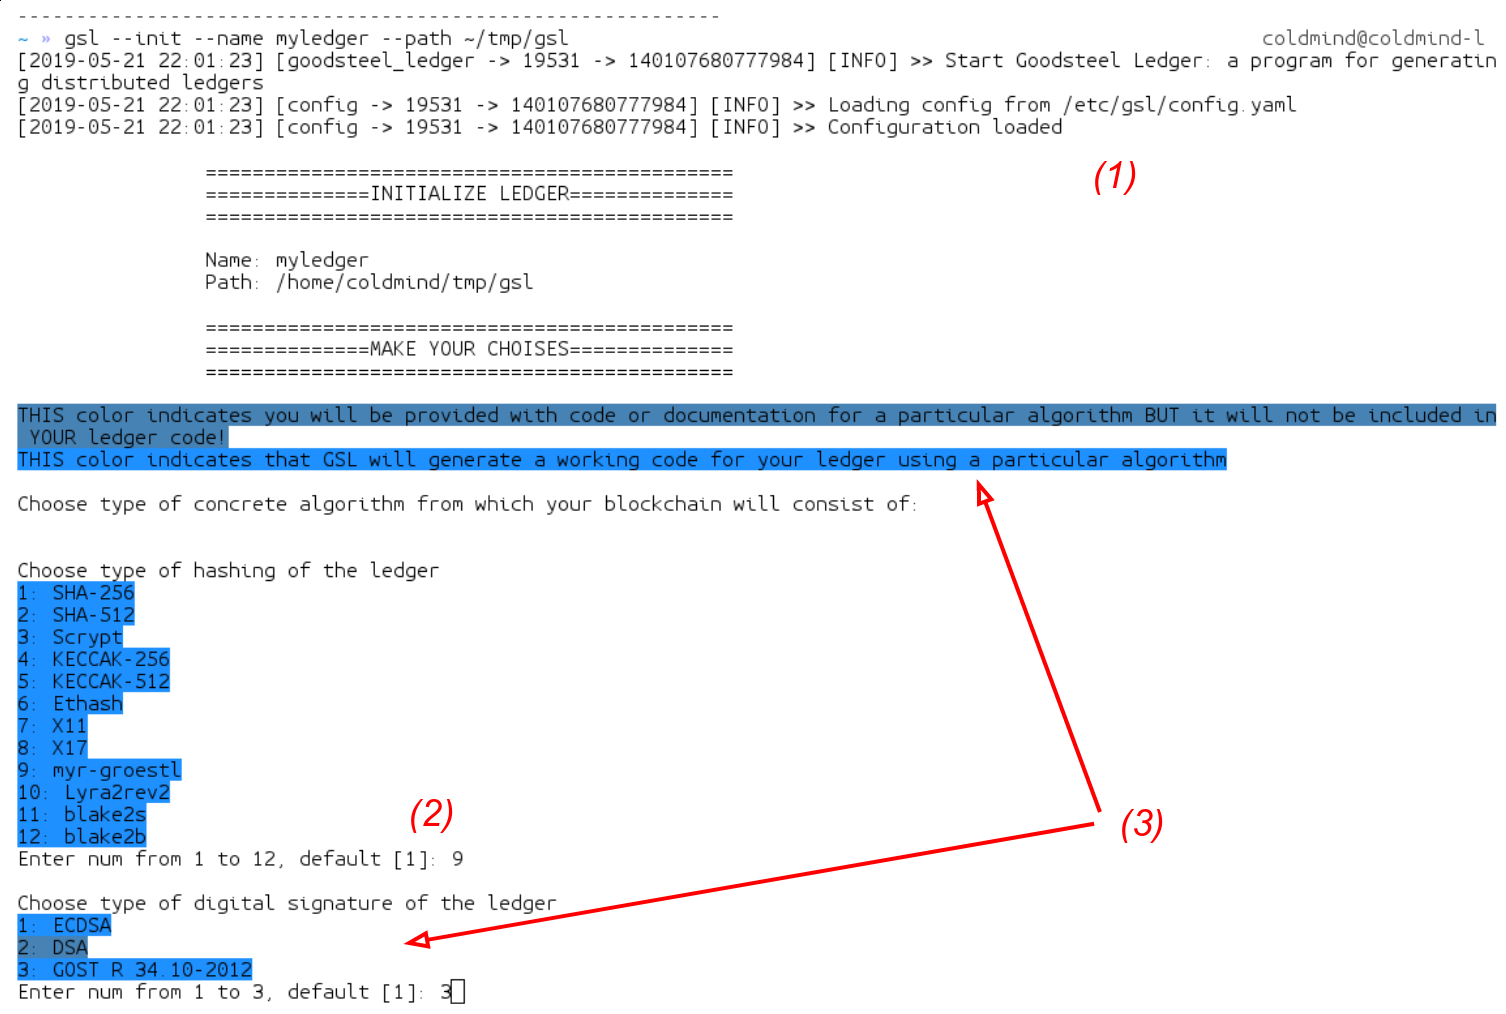
\includegraphics[width=0.85\textwidth]{./screenshots/algs_choose}
    \caption{Начало работы компоновщика}\label{algs_choose}
\end{figure}

Алгоритмы должны отображаться пронумерованно; по категориям (Рис.~\ref{algs_choose})

Вывод алгоритмов должен быть в цвете, обозночающим степень поддержки программой
алгоритма (пункт 3 Рис.~\ref{algs_choose})

Должен поддерживаться выбор алгоритмов ``по умолчанию'', и при отсутствии ввода
определённого номера алгоритма, выбираться указанный в качестве алгоритма ``по
умолчанию'' (пункт 2 Рис.~\ref{algs_choose})

\begin{figure}[h!]
    \centering
    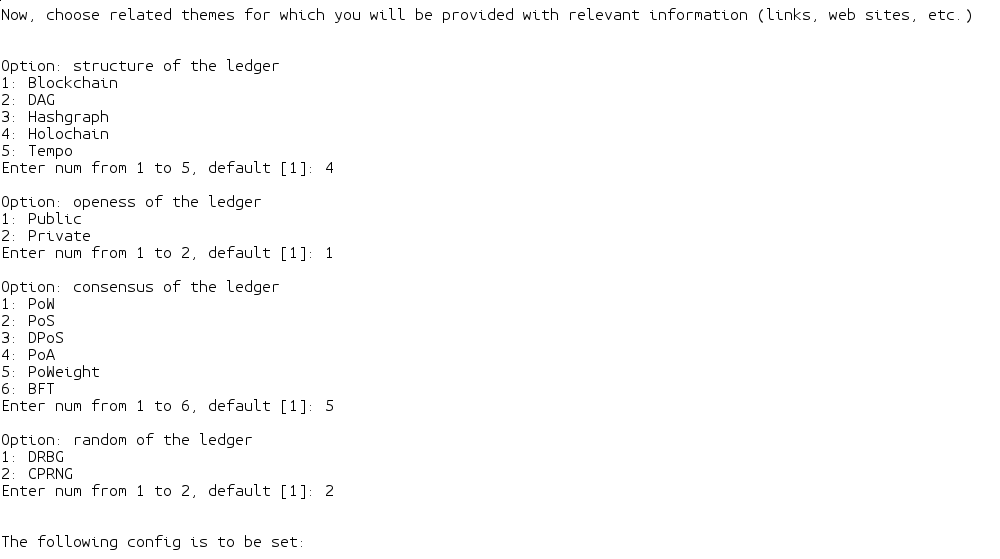
\includegraphics[width=\textwidth]{./screenshots/additional_opts}
    \caption{Вывод опций по которым будет дана справочная информация}\label{additional_opts}
\end{figure}

После выбора алгоритмов хэширования и цифровой подписи, пользователю должны
показываться свойства/структура/другие алгоритмы распределённых реестров, по
которым можно получить справочную информацию (Рис.~\ref{additional_opts})

\begin{figure}[h!]
    \centering
    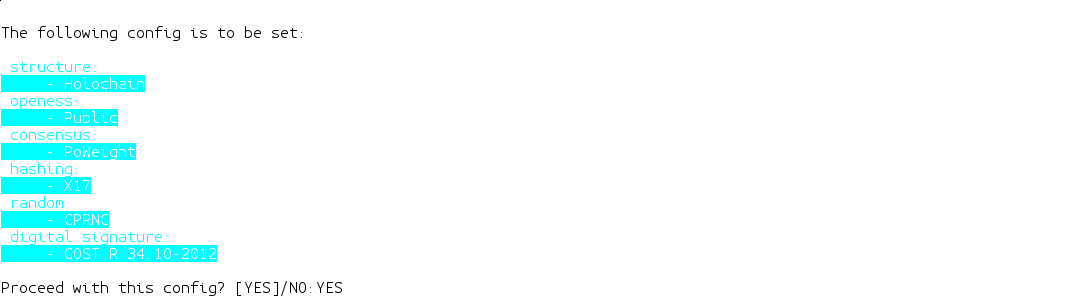
\includegraphics[width=\textwidth]{./screenshots/confirmation}
    \caption{Подтверждение выбранных опций}\label{confirmation}
\end{figure}

Должен выводиться итоговый выбор пользователя с вопросом о намерении принять
изменения и продолжить дальнейшее выполнение программы
(Рис.~\ref{confirmation})

\begin{figure}[h!]
    \centering
    \minipage{0.49\textwidth}
    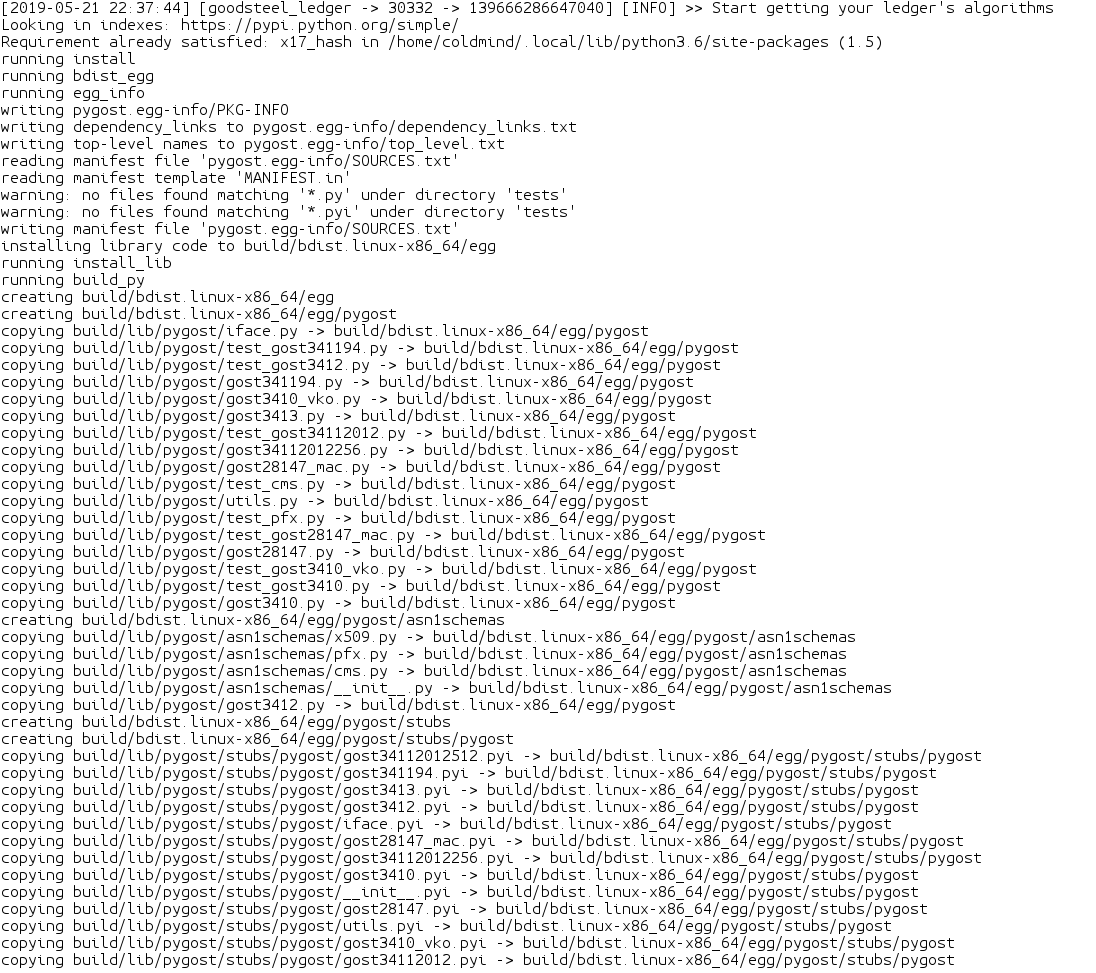
\includegraphics[width=\textwidth]{./screenshots/installing1}
    \caption{Процесс установки выбранных алгоритмов}
    \label{inst1}
    \endminipage\hfill
    \minipage{0.49\textwidth}
    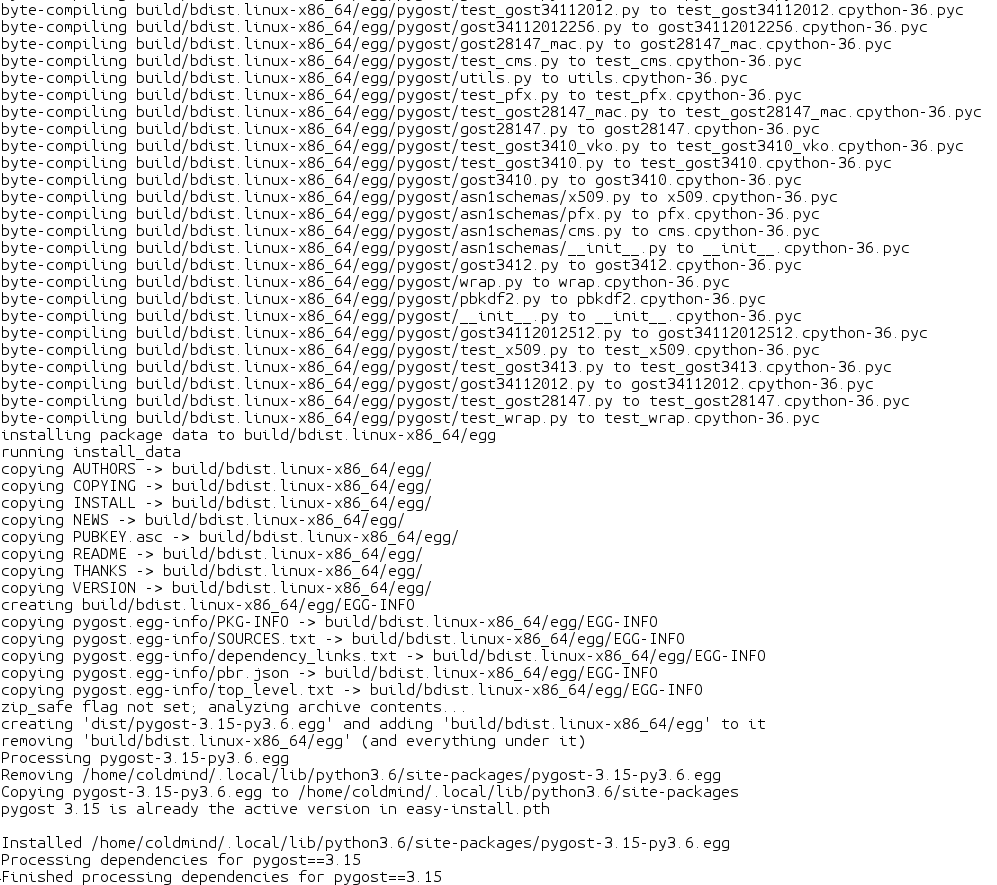
\includegraphics[width=\textwidth]{./screenshots/installing2}
    \caption{Завершение установки выбранных алгоритмов}
    \label{inst2}
    \endminipage{}
\end{figure}

При подтверждении выбора набора алгоритмов пути до исходных кодов алгоритмов
должны быть получены из хранилища, и по ним должна произойти установка в
систему (Рис.~\ref{inst1}~-~\ref{inst2}).

\begin{figure}[h!]
    \centering
    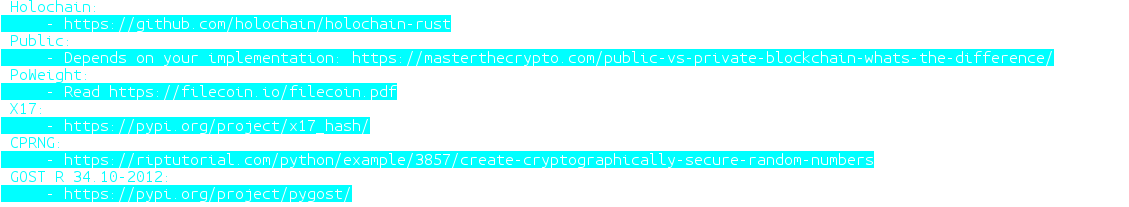
\includegraphics[width=\textwidth]{./screenshots/spravka}
    \caption{Справочная информация в конце выполнения компоновщика}\label{spravka}
\end{figure}

По завершении выполнения программа должна выводить справочную информацию по
выбранным свойствам распределённого реестра (Рис.~\ref{spravka}).

\begin{figure}[h!]
    \centering
    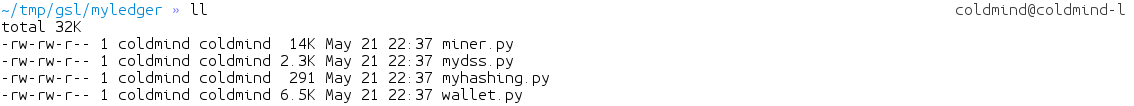
\includegraphics[width=\textwidth]{./screenshots/lldir}
    \caption{Директория со сгенерированным кодом}\label{lldir}
\end{figure}

После завершения работы программы по указанной директории должны располагаться
модули {\small wallet.py} и {\small miner.py} вместе с выбранными алгоритмами
хэщирования и электронной подписи (Рис.~\ref{lldir}).

Должно производиться автообновление алгоритмов каждый день в 21:00. Каждый день
в репозитории проекта должен быть коммит в 21:00 с обновлениями алгоритмов,
если таковые имеются.


\subsubsection{Проверка требований к реализации блокчейна}
Проверка реализованного функционала продемонстрирована на скриншотах ниже.
Модуль {\small wallet.py} будем называть \textbf{кошелёк}, а {\small miner.py}
--- \textbf{майнер}.

\begin{figure}[h!]
    \centering
    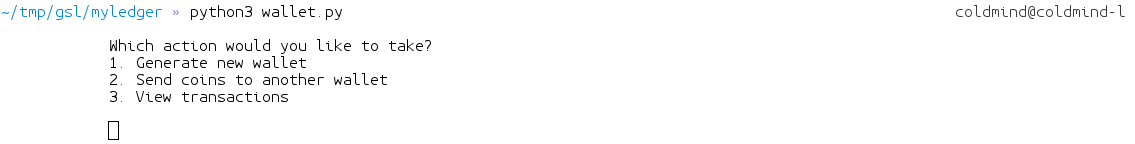
\includegraphics[width=\textwidth]{./screenshots/wallet_options}
    \caption{Возможности кошелька}\label{wallet}
\end{figure}

Возможности кошелька должны включать в себя 3 функции: генерирования нового
адреса (пары публичный и приватный ключ), отправки средств с одного адреса на
другой, а так же просмотр блокчейна (Рис.~\ref{wallet}).

\begin{figure}[h!]
    \centering
    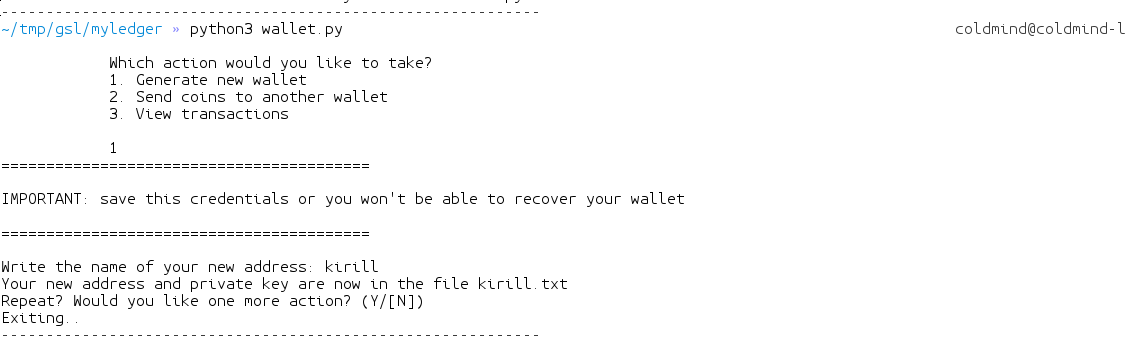
\includegraphics[width=\textwidth]{./screenshots/gen_kirill}
    \caption{Генерация адреса {\small kirill}}\label{gen_kirill}
\end{figure}

При выборе первой опции должен отображаться диалог с требованием ввести имя, и
дальнейшей генерацией адреса кошелька (пары публичный-приватный ключи) (Рис.~\ref{gen_kirill})

\begin{figure}[h!]
    \centering
    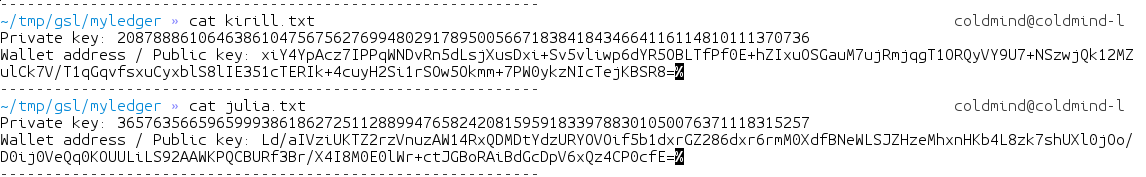
\includegraphics[width=\textwidth]{./screenshots/cat}
    \caption{Просмотр сгенерированных адресов кошельков}\label{cat}
\end{figure}

Адрес кошелька должен записываться в файл с расширением {\small .txt} и
указанным именем в названии (Рис.~\ref{cat}).

\begin{figure}[h!]
    \centering
    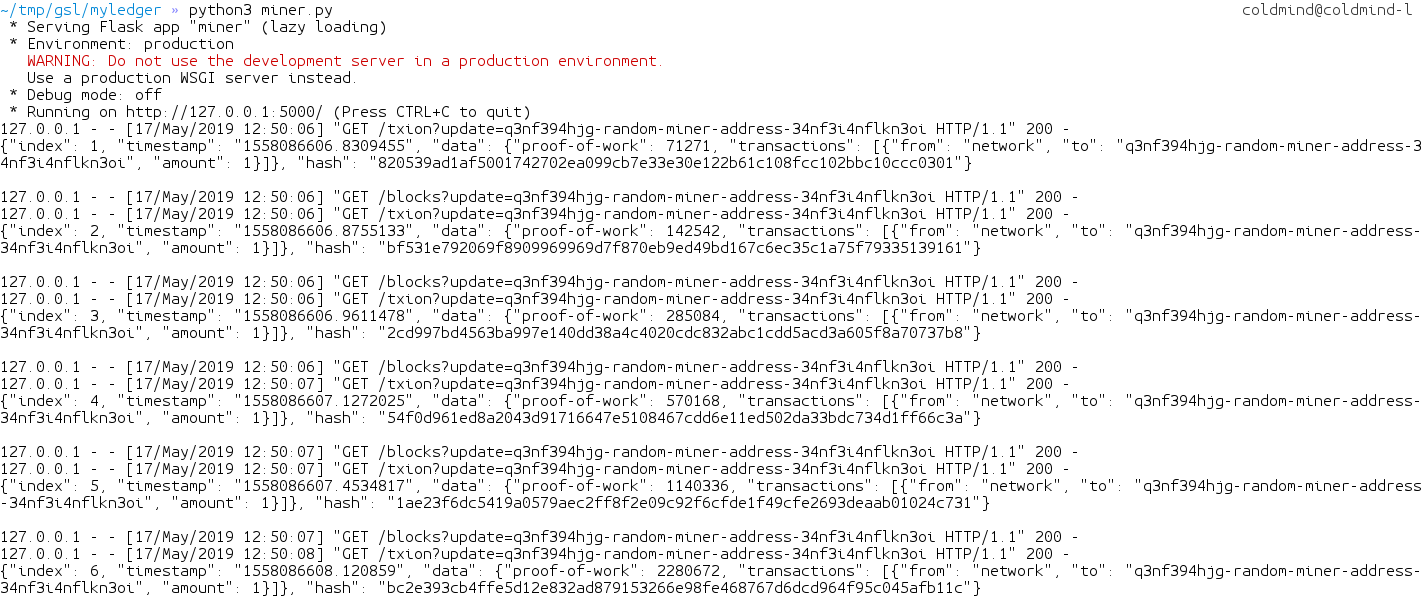
\includegraphics[width=\textwidth]{./screenshots/miner_run}
    \caption{Лог работы майрена}\label{log1}
\end{figure}

\begin{figure}[h!]
    \centering
    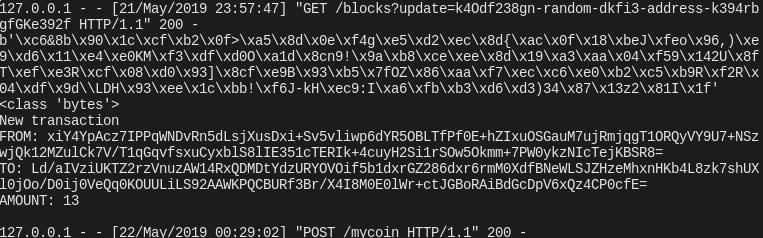
\includegraphics[width=\textwidth]{./screenshots/log_send}
    \caption{Лог регистрации новой транзакции}\label{log2}
\end{figure}

При запуске майнера, должен вестись лог о проведённых транзакциях и их
валидациях (Рис.~\ref{log1}~-~Рис.~\ref{log2}).

\begin{figure}[h!]
    \centering
    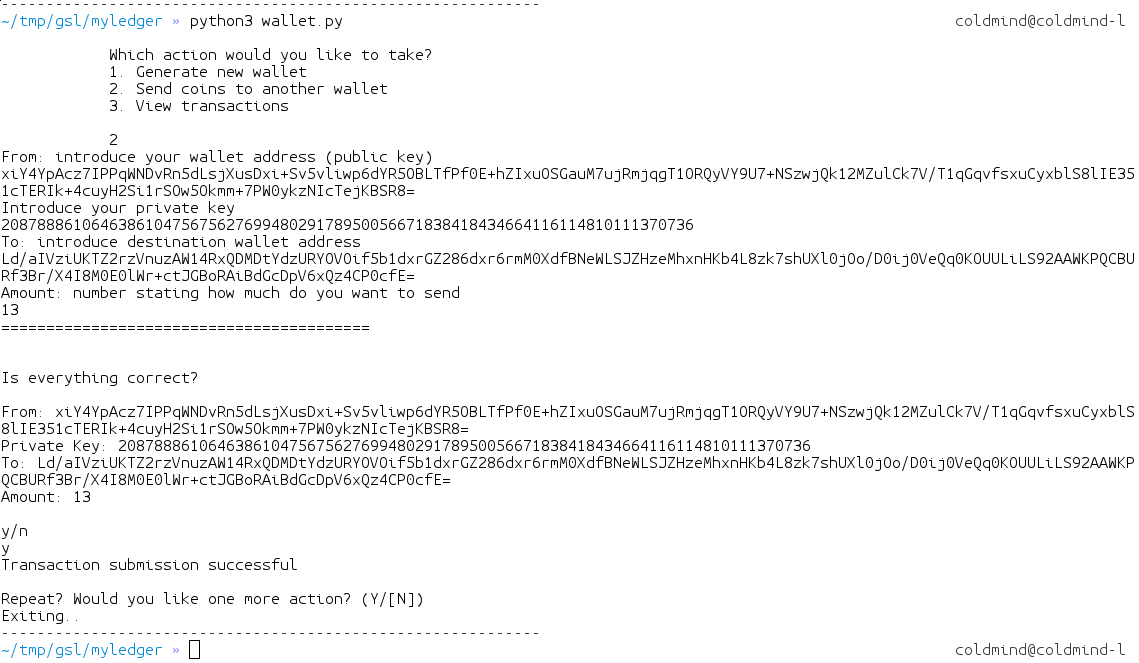
\includegraphics[width=\textwidth]{./screenshots/sending}
    \caption{Процесс отправки средств}\label{sending}
\end{figure}

В кошельке при отправке условных средств с одного счёта на другой, должны
требоваться публичный и приватный адреса отправителя, а так же публичный ключ
получателя (Рис.~\ref{sending}).

\begin{figure}[h!]
    \centering
    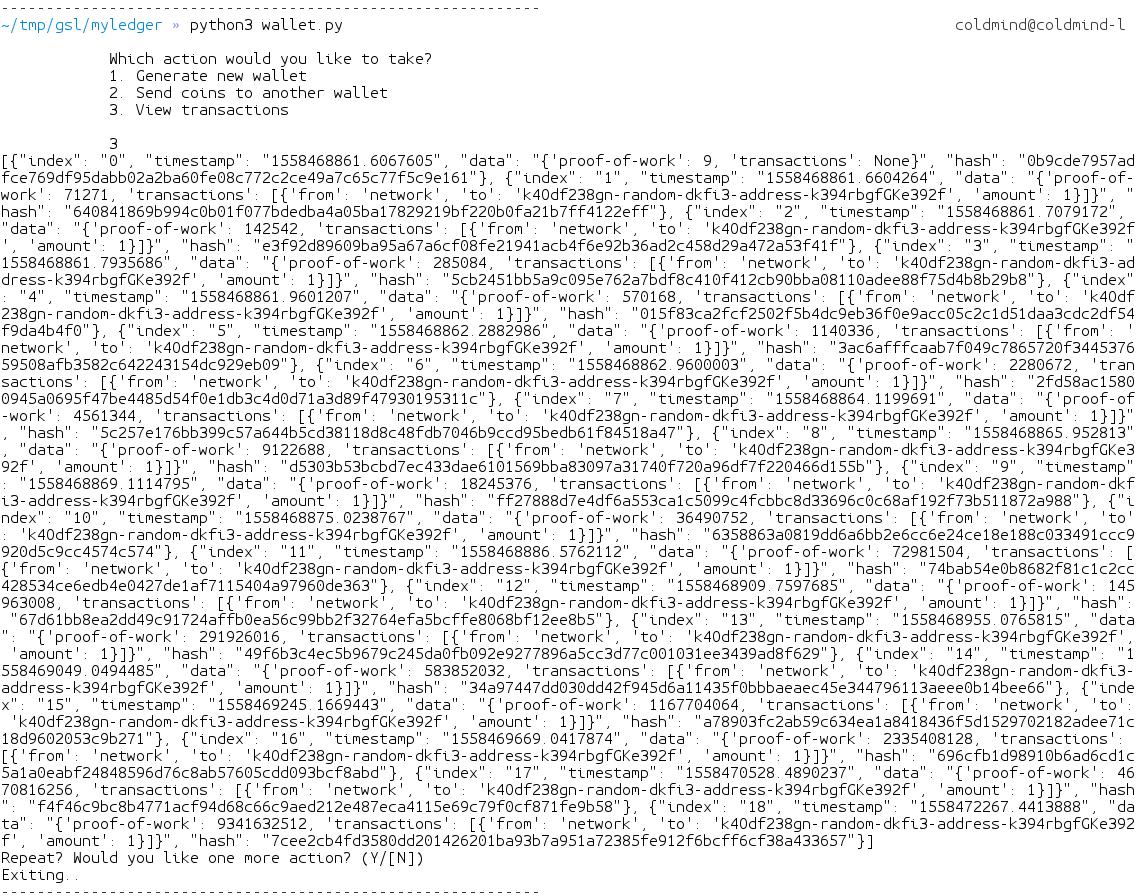
\includegraphics[width=\textwidth]{./screenshots/full_chain}
    \caption{Отображение полной цепочки транзакций}\label{full_chain}
\end{figure}
При выборе третей опции в кошельке, должен отобразиться полная цепочка
транзакций (блокчейн) (Рис.~\ref{full_chain}).

\newpage
\subsection{Проверка требований к временным характеристикам}
\subsubsection{Проверка требований к компоновщику}
Время запуска приложения не должно превышать 1.05 секунд (Рис.~\ref{launch})

\begin{figure}[h!]
    \centering
    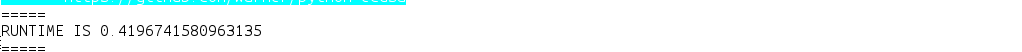
\includegraphics[width=0.7\textwidth]{./screenshots/runtime}
    \caption{Лог замера времени}
    \label{launch}
\end{figure}

Все временные требования должны быть соблюдены.
\subsubsection{Реализация блокчейна}
Временные требования к работе реализации блокчейна (майнера и кошелька) не предъявлялись.


\newpage
\section{Приложение 1. Терминология}
\subsection{Терминология}
\begin{description}
    \item[Активность (Activity)] ---
        Activity — это компонент приложения, который выдает экран, и с которым
        пользователи могут взаимодействовать для выполнения каких-либо
        действий, например набрать номер телефона, сделать фото, отправить
        письмо или просмотреть карту. 

    \item[Фрагмент (Fragment)] ---
        Фрагмент (класс Fragment) представляет поведение или часть
        пользовательского интерфейса в операции (класс Activity). В одной
        активности может быть несколько фрагментов.

    \item[crawler] ---
            Программный модуль, работающий в фоне и производящий сбор данных с сайтов
            указанных магазинов, с последующей отправкой их на сервер в формате
            JSON

    \item[Пользовательский товар] ---
            Товар, представленный в виде текста, имеющий в себе массив товаров,
            подходящих при сопоставлении названий к данному. Пример.
            Пользовательский товар ``Сок'' имеет массив сопоставившихся товаров [Сок
            Добрый 1л Яблоко; Сок J-7 апельсин с мякотью].

    \item[Spider] ---
        Часть crawler'a, отвечающая за непосредственный сбор информации с
        веб-страниц, переход между страницами и дальнейшую отправку собранных
        данных другим модулям crawler'a.

    \item[log-сообщения] ---
        Сообщения, которые выводит система для подробного отслеживания
        происходящих в ней процессах. Обычно содержит точное время процесса,
        тэг процесса, и информативное сообщение.

\end{description}



\newpage
\section{Приложение 2. Список используемой литературы}
% \nocite{*}
% \printbibliography{}



% Index
\newpage
\eskdListOfChanges

% \phantomsection
% \addcontentsline{toc}{section}{Алфавитный указатель}
% \printindex

\end{document}
